%%%%%%%%%%%%%%%%%%%%%%%%%%%%%% -*- Mode: Latex -*- %%%%%%%%%%%%%%%%%%%%%%%%%%%%
%% 12-17.tex --  Tech report on RAs
%% Author          : Philip Johnson
%% Created On      : Mon Sep 23 11:52:28 2002
%% Last Modified By: Philip Johnson
%% Last Modified On: Mon Jun 14 12:41:23 2010
%%%%%%%%%%%%%%%%%%%%%%%%%%%%%%%%%%%%%%%%%%%%%%%%%%%%%%%%%%%%%%%%%%%%%%%%%%%%%%%
%%   Copyright (C) 2009 Philip Johnson
%%%%%%%%%%%%%%%%%%%%%%%%%%%%%%%%%%%%%%%%%%%%%%%%%%%%%%%%%%%%%%%%%%%%%%%%%%%%%%%
%% 

\documentclass[]{article}
\usepackage{graphicx}
\usepackage{cite}
\usepackage{url}
\usepackage{enumitem}
\usepackage{times}
\usepackage[margin=1in]{geometry}

% uncomment the % away on next line to produce the final camera-ready version
% and uncomment the \thispagestyle{empty} following \maketitle
%\pagestyle{empty}
\begin{document}

%\onecolumn
%\setlength{\parindent}{0cm}


\title{{\bf Looking under the lamppost for useful software analytics}} 

\author{Philip M. Johnson\\
        Collaborative Software Development Laboratory\\
        Department of Information and Computer Sciences\\
        University of Hawai`i at M\=anoa\\
        Honolulu, HI 96822\\
        johnson@hawaii.edu\\
}


\maketitle

\thispagestyle{empty}


\setlength{\parskip}{3pt plus 1pt minus 1pt} 

\section{Introduction}
Noam Chomsky once said, {\em ``Science is a bit like the joke about the drunk who is
  looking under a lamppost for a key that he has lost on the other side of the street,
  because that's where the light is. It has no other choice.'' \cite{Barsky98}} For over
15 years, researchers at the Collaborative Software Development Laboratory at the
University of Hawaii have looked for analytics that aid in understanding and
improving the process of software development, and we believe Chomsky's scientific
lamppost provides a useful metaphor for understanding both our efforts and those of many
other researchers in this area.

When it comes to analytics regarding software development, we claim that
``looking under the lamppost'' is roughly equivalent to ``collecting and analyzing metrics
that are easy to obtain with little social, political, or developmental impact.''  In
other words, the easier and less controversial a software analytic for software
development, the more constrained its usefulness and generality.  For example, the data
contained in a configuration management repository is easy to collect and the
intrinsically public nature of the repository means that few developers will object to
such collection and analysis, but such analytics provide an extremely narrow range of data
regarding development activities, which intrinsically limits the kinds of analytics that
result.  On the other hand, the original version of the Personal Software Process yields
extremely rich and impactful analytics, but entails significant overhead on developers and
the analytics themselves have significant social and political implications.

This article provides an ``illustrated tour'' through over 15 years of research and
development of analytics for software development. When put together with current trends
in the field, it provides a portrait of the various trade-offs that must be made between
light and insight in the search for useful information about software development
processes and products.

\section{It is better to light a candle: The Personal Software Process}

Our research on software analytics for software development began in 1996 when we began
using and evaluating the Personal Software Process (PSP) as described in Watts Humphrey's
``A Discipline for Software Engineering'' \cite{Humphrey95}. This book was innovative in
several dimensions: it showed how organizational software process analytics could be
adapted to individual developers, it showed how these analytics could be used to drive
improvement, and it presented the practices in an incremental fashion amenable to
academic and professional adoption. 

\begin{figure}[!tb]
\centering
\includegraphics[width=0.95\columnwidth]{defects.eps}
\caption{Sample Defect Recording Log. In the PSP, even compiler (syntax) errors are recorded.}
\label{fig:defect-log}
\end{figure}
 
This version of the PSP uses simple spreadsheets, manual data collection, and manual
analysis. The effort required to collect and manage this data is substantial: in one
version of the PSP, developers must fill out 12 separate forms, including a project plan
summary, a time recording log, a defect recording log, a process improvement proposal, a
size estimation template, a time estimation template, a design checklist, and a code
checklist. These forms typically yield over 500 distinct values that must be manually
calculated by the developer.  Interestingly, Humphrey actively embraced the manual nature
of the PSP, writing on page 217 that {\em ``It would be nice to have a tool to
  automatically gather the PSP data. Because judgement is involved in most personal
  process data, no such tool exists or is likely in the near future''}.  More
fundamentally, however, is the fact that Humphrey viewed his PSP processes as simply a
bootstrapping method: in Chapter 13, ``Defining the Software Process'', he exhorts
developers to modify the forms and procedures presented earlier in order to address their
specific circumstances and needs. That chapter presents a form developed by the author for
his personal use and labelled PSP7, five versions higher than the final version presented
in the book (PSP 2.1).

From the perspective of our metaphor, we view this original version of the PSP as
``lighting a candle'' because the approach is designed to develop custom,
situationally-specific analytics. The manual nature of the PSP makes its analytics
fragile, in the same way that a candle flame is easy to extinguish, but just like a candle
enables its holder to navigate in the darkness, the PSP enables and encourages its users
to search for the analytics best suited to their needs.  As a simple example, consider a
developer who suspects that the number of interruptions she experiences each morning
directly impacts on her productivity.  The PSP provides both explicit encouragement to
explore such analytics and a relatively low cost means to do so.

After two years using and teaching the predefined PSP processes, we began to suspect that
the manual nature of the PSP created the potential for significant data quality problems,
and performed an empirical study that explored this issue by checking over 30,000 data
values generated by classroom use of the PSP \cite{csdl-98-11}. We found that the manual
nature of the PSP could sometimes lead to incorrect process conclusions even though the
overall error rate was very low---less than 5\%.  To address this problem, we embarked
upon a new research project called Project LEAP, and in retrospect, unwittingly
compromised one of the best features of the PSP.

\section{Project LEAP: From candle to campfire} 

Project LEAP (Lightweight, Empirical Anti-measurement dysfunction, and Portable) attempted
to address the data quality problems we encountered with the manual PSP through the
development of a toolkit to automate and normalize data analysis \cite{csdl-99-08}.  
While the developer was still required to enter most data by hand, the toolkit automated
the subsequent PSP analyses and in some cases provided alternative analyses (such as
various forms of regression) not explored in the PSP.  It claimed a ``lightweight''
approach by not prescribing the sequence of activities followed by developers (as in the
PSP). It attempted to avoid measurement dysfunction by enabling developers to control
their data files, by maintaining data about only one developer's activities, and by not
referencing developer names in the data files. Finally, LEAP data was intended to be
portable: a source of personal process data that the developer could keep with them as
they moved from project to project and organization to organization.  Figure
\ref{fig:leap} illustrates one of the toolkit components, which supports time estimation
based upon personal historical data and selection of a regression analysis.

\begin{figure}[!tb]
\centering
\includegraphics[width=0.50\columnwidth]{planword.eps}
\caption{The time estimation toolkit component in Project LEAP.}
\label{fig:leap}
\end{figure}

Returning to our metaphor, Project LEAP can be viewed as replacing the PSP candle with a
``campfire''.  The introduction of higher level tool support metaphorically increases the
light by improving data quality and lowering the amount of manual analysis.  On the other
hand, unlike a candle, whose light can be moved around easily according to the interests
of the holder, a campfire is stationary: participants must come to it.  By introducing
automation, Project LEAP makes certain analytics easy to collect but others
disproportionately difficult.  Consider our hypothetical developer who suspects that
interruptions are impacting on her productivity: she would now be expected to design and
implement a new Leap toolkit component as opposed to a simple spreadsheet form. 

The LEAP toolkit was actively developed from 1997 to 2001, and was downloaded and used in
many classroom and industrial settings.  Industrial developers commented that they were
attracted to the fact that the toolkit offered much of the analytics associated with the
PSP without dictating the development process.  In 2001, the Agile Manifesto
\cite{AgileManifesto} was published, defining a name and set of principles that appeared
to stand in direct opposition to the PSP's commitment to process definition, adherence,
and high-overhead data collection and analysis.

After several years of using the LEAP toolkit, we came to agree with Humphrey that the PSP
approach could never be fully automated and would inevitably require a significant amount
of manual data entry.  We also came to agree with the Agile community that such overhead
frequently introduced excessive overhead into development without providing enough return
on investment, particularly when each project was sufficiently different from previous as
to render historical data inappropriate for comparison.

What we decided to try to do, however, departed from the conventional wisdom of both
camps. Unlike the PSP/TSP community, we would abandon any pretense of supporting PSP
analyses.  Unlike the agile community, we would continue to embrace measurement and
analysis.  Our research goal was simple to state: what kinds of useful software analytics
could be obtained if both collection and analysis were ``free''?  This goal became the
mission of a decade-long research project called Hackystat. 

\section{Hackystat:  The harsh glare of operating room lights}

As users of both the manual PSP as well as the LEAP toolkit, we were personally aware of
the overhead on development created by such data collection, even though there was
significant evidence for downstream benefits in the form of better planning and reduced
defects. The conventional wisdom, as prescribed by methodologies such as GQM
\cite{Basili94gqm}, is to define high-level goals first and then figure out the data
collection and analysis necessary to achieve them.  In the Hackystat research project
\cite{csdl2-02-07}, we chose to work in the opposite direction: we first focused on
developing ways to collect software process and product data with little to no overhead to
developers, and then explored what high-level software engineering goals could be
supported by analyses on this data. Hackystat implements a service-oriented architecture,
where sensors attached to development tools gather process and product data and send it
off to a server which can be queried by other services to build higher level analyses. 

Some of the important design features of Hackystat relevant to this discussion include:
\begin{itemize}
\item {\em Client as well as server-side data collection.}  Modern software development
  typically includes activities undertaken by individual developers on their local
  workstation as well as server (or cloud)-based activities. From the start, we developed
  instrumentation for client-side tools such as editors, build tools, test tools, as well
  as server-side tools such as configuration management repositories, build servers, etc.
\item {\em Unobtrusive data collection.}  One of the most frustrating aspects of manual data
  collection is the ``do some work, then interrupt your work to record what you worked on''
  loop. An important requirement for Hackystat was to make data collection as unobtrusive
  as possible: you should not notice that data is being collected, and the system should
  not make assumptions about network availability. For example, Hackystat client-side
  instrumentation locally caches any data collected while a developer is working
  offline, then sends the data to the Hackystat data repository once the developer
  reconnects. 
\item {\em Fine-grained data collection.}  By instrumenting client-side tools, we could
  collect data on a minute-by-minute or even second-by-second basis. For example, one type
  of data collection possible in Hackystat is called ``Buffer transition'', where a data
  instance is collected each time the developer changes the active buffer from one file to
  another.
\item {\em Both personal and group-based development.}  In addition to tracking ``personal''
  development data, developers can define projects
  and shared artifacts to represent group work.  
\end{itemize}

During the past ten years, we have discovered significant technical strengths as well as
significant political and social weaknesses in this approach.  Technically, Hackystat has
led to a broad variety of innovations, including the development of a toolkit for defining
and visualizing software project ``telemetry'' \cite{csdl2-04-11}, support for high
performance computing software development \cite{csdl2-04-22}, a method for prioritizing
what software development artifacts to inspect \cite{csdl2-05-01}, an operational
definition for Test-Driven Development providing a means to automatically assess when
developers are using it \cite{csdl2-09-01}, an approach to software process discovery
\cite{csdl2-10-09}, and a mechanism called the ``Software ICU'' for assessing the health
of an individual project both alone and in relation to other projects \cite{csdl2-09-02}.
Figure \ref{fig:icu} shows an image from this Hackystat-based system.

\begin{figure}[!tb]
\centering
\includegraphics[width=1.0\columnwidth]{portfolio-2008.eps}
\caption{A software intensive care unit display, based on Hackystat.}
\label{fig:icu}
\end{figure}


In addition to discovering the technical possibilities of systems built with Hackystat, we
also discovered significant social and political problems.  First, the unobtrusive nature of
data collection, which we viewed as a feature, was to some developers a bug: they did not
want to install instrumentation into their environment that would collect data regarding
their activities without telling them about it.  Second, the client-side, fine-grained
data collection has the potential to create discord within a development group: one
student referred to the Software ICU as ``hacky-stalk'', complaining about the
transparency it provided about each member's working style.  Third,
the client-side, fine-grained data that enabled the most compelling analytics about
development was simultaneously the largest obstacle to industrial adoption of Hackystat
technologies: developers repeatedly informed us that they were not comfortable with
collection of such data, despite management promises to use it appropriately. Robert
Austin provides much more details on this phenomena and its typical outcome of
``measurement dysfunction'' \cite{Austin96}.

To better understand these problems, it is helpful to take a closer look at the Software
ICU.  As shown on the left side of Figure \ref{fig:icu}, the Software ICU collects and
displays structural metrics about software artifacts, such as coverage, complexity,
coupling, and churn, and the Software ICU colors their most recently observed values and
their trends over time with red, yellow, or green to indicate their ``health''.  Another
structural metric is size, which the Software ICU displays for informational purposes but
presents in white (because the analysis has no way of characterizing current size or size
trends over time as ``healthy'' or ``unhealthy''.)  The Software ICU displays these values
for a portfolio of projects, allowing comparison of project data.  In general, collection,
analysis, and public presentation of the values to the left of the (white) Size data is
not controversial.

It is on the right side of the Software ICU interface where things get interesting, as
this side presents four indicators of ``health'' based upon aggregations of individual
developer behavior: DevTime, Commit, Build, and Test.  DevTime measures how much time each
developer spends in their IDE working on the project; Commit measures how often each
developer commits to the repository (and how many lines of code are committed each time);
Build measures how many times each developer builds the system (and whether the build is
successful); and Test measures how often each developer invokes the test suite on the
system (and whether the tests ran successfully).  In the Software ICU, clicking on any of
the sparklines results in a drilldown to a more detailed perspective. For example,
clicking on the DevTime sparkline generates a visualization showing the individual DevTime
of each developer.

While our research provides evidence that such representation of individual developer
behavior makes some uncomfortable, it is also necessary if one is to provide certain kinds
of insight.  As a simple example, an aphorism of agile software development is ``build
early and often'', and the Software ICU can actually measure the extent to which
developers adhere to this principle.  More interestingly, the Hackystat-based Zorro system
can automatically determine whether or not and the extent to which developers use
test-first design methods (popularly known as the ``red/green/refactor'' cycle).

From the perspective of our metaphor, Hackystat could be viewed as high intensity
operating room lights. The approach provides the potential for abundant illumination and
deep insight, but these benefits cannot be achieved without procedures some might view as
``invasive''.

\section{The state of practice: back under the lamppost}




\section{Misc}

The PSP became quite popular in the late 1990's, was enhanced to support group work as the
``Team Software Process'', and certification programs and conferences were established
under the stewardship of the Software Engineering Institute.  



\section{Acknowledgements}

Acknowledge the various NSF grants. 

\bibliographystyle{plain}
\bibliography{csdl-trs,psp,hackystat,12-11}
\end{document}
